\documentclass[10pt,twocolumn]{article}
\usepackage{graphicx}
\usepackage{amsmath}
\usepackage{float}
\usepackage{hyperref}
\usepackage{geometry}

% Réglages compacts
\geometry{margin=1.6cm, columnsep=1.1cm}
\setlength{\parskip}{0pt}
\setlength{\parindent}{1em}

\title{\textbf{Analyse temporelle, structurelle et communautaire du réseau hospitalier} \\
\large Centralités, modèles nuls, temporalité et organisation core--périphérie}
\author{Projet Graph Mining}
\date{}

\begin{document}
\maketitle

% ============================================================
\section{Introduction}
% ============================================================

Ce rapport analyse un réseau de contacts mesuré en milieu hospitalier,
où les interactions entre individus (personnel médical, personnel administratif
et patients) ont été enregistrées sur une période continue.
Après agrégation des contacts, le réseau étudié est composé de
\textbf{75 nœuds} et \textbf{1139 arêtes}, chaque arête pouvant être pondérée
par la durée cumulée des interactions.

L’analyse vise à décrire la structure effective du réseau hospitalier
et à identifier les individus jouant un rôle central dans les interactions.
Nous étudions successivement les centralités, la comparaison avec des graphes modèles,
la dynamique temporelle des contacts et l’organisation communautaire et hiérarchique
du réseau.




% ============================================================
\section{Mesures de centralité}
% ============================================================

\subsection{Degree centrality}

Les degrés les plus élevés sont observés chez les infirmiers \textbf{NUR},
avec des valeurs atteignant \textbf{58} et \textbf{57} voisins (IDs 1193, 1164, 1115),
suivis par certains médecins \textbf{MED} (jusqu’à \textbf{53}).
Ces individus correspondent aux principaux hubs du réseau,
en interaction avec un grand nombre d’acteurs distincts.

\subsection{Strength}

Le cumul des durées de contacts est largement dominé par les \textbf{NUR}.
Les valeurs de strength les plus élevées dépassent \textbf{4000}
(ID 1115 : \textbf{4286}, ID 1210 : \textbf{4077}),
confirmant que les infirmiers concentrent les interactions les plus longues
et les plus fréquentes.

\subsection{Betweenness centrality}

Les valeurs de betweenness les plus importantes concernent principalement
des \textbf{NUR} (jusqu’à \textbf{0.0708} pour l’ID 1210),
ainsi que quelques \textbf{ADM} et \textbf{MED}.
Ces individus jouent un rôle d’intermédiaire entre différentes parties du réseau.

\subsection{Closeness centrality}

Les scores de closeness les plus élevés sont également observés
chez les \textbf{NUR}, avec des valeurs supérieures à \textbf{0.40}
(ID 1210 : \textbf{0.4088}),
ce qui reflète leur position centrale et leur proximité moyenne
au reste du réseau.

\subsection{Eigenvector centrality}

L’eigenvector centrality met en évidence un noyau fortement interconnecté
dominé par les \textbf{NUR}.
Les valeurs maximales atteignent \textbf{0.49} (IDs 1115 et 1210),
indiquant une forte connexion à d’autres nœuds eux-mêmes centraux.

\subsection{PageRank}

Le PageRank pondéré par la durée des contacts confirme ces observations.
Les scores les plus élevés sont obtenus par des \textbf{NUR},
avec des valeurs allant jusqu’à \textbf{0.0558} (ID 1115),
recouvrant largement les individus identifiés par le strength.

\subsection{Interprétation des centralités}

L’ensemble des mesures converge vers le même constat :
les \textbf{NUR}, puis les \textbf{MED}, occupent les positions les plus centrales
du réseau, à la fois en nombre de contacts, en durée cumulée
et en importance structurelle globale.
À l’inverse, les \textbf{PAT} et \textbf{ADM} apparaissent plus souvent
en périphérie, avec des niveaux de connectivité et d’influence plus faibles.


% ============================================================
\section{Comparaison avec des graphes modèles (null models)}
% ============================================================

L’objectif ici est de déterminer si les propriétés observées sont explicables par  le hasard pur (Erd\H{o}s--R\'enyi) ou par la seule distribution des degrés (Configuration Model).

\subsection{Erd\H{o}s--R\'enyi : hétérogénéité et hubs}

Le modèle ER $G(N,q)$ produit une distribution de degrés proche d’une loi de Poisson (concentrée autour du degré moyen).  
Or, le réseau réel est beaucoup plus \textbf{hétérogène} : il présente une queue plus lourde et des hubs marqués.

\begin{figure}[H]
\centering
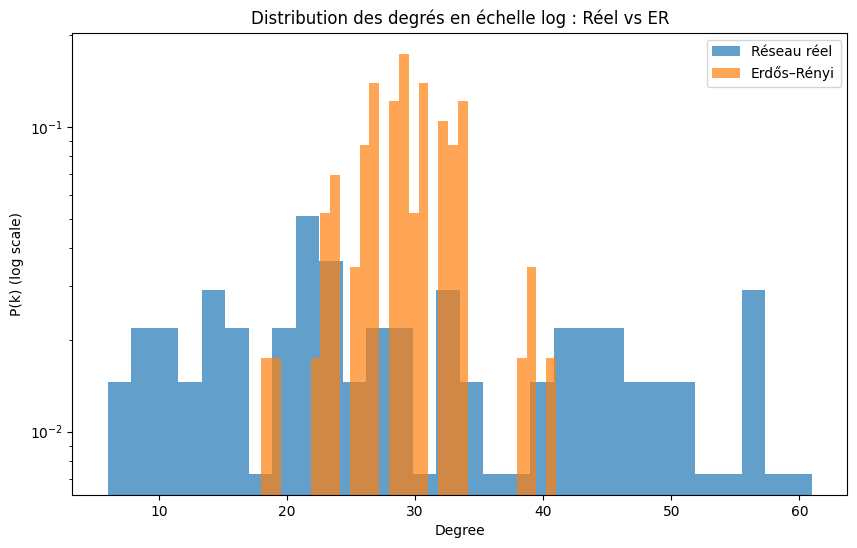
\includegraphics[width=0.90\linewidth]{images/article1/image1.png}
\caption{Distribution des degrés : réseau réel vs Erd\H{o}s--R\'enyi.}
\end{figure}

Conclusion : un graphe aléatoire simple ne peut pas reproduire l’organisation hospitalière.

\subsection{Configuration Model : triangles et organisation par rôle}

Le Configuration Model conserve la séquence de degrés, mais randomise les connexions.  
On observe alors des écarts structuraux importants :

\begin{itemize}
    \item \textbf{Clustering} : le réseau réel présente un clustering nettement plus élevé ($\approx 0.64$) que le CM ($\approx 0.40$), indiquant une forte présence de triangles liés aux équipes et aux soins répétés.
    \item \textbf{Distance moyenne} : légèrement plus faible dans le réseau réel ($1.59$ contre $1.70$), suggérant une connectivité renforcée via quelques individus centraux.
    \item \textbf{Assortativité par rôle} : négative dans le réseau réel ($r=-0.12$) et quasi nulle dans le CM, montrant que les interactions NUR--PAT et MED--PAT reflètent des contraintes fonctionnelles plutôt que la seule distribution des degrés.
\end{itemize}


\subsection{Interpretation des  modèles}

Le contrôle de la distribution des degrés ne suffit pas à reproduire la structure observée.
Le réseau réel reste caractérisé par une forte densité locale, des interactions dépendantes des rôles et une organisation non aléatoire liée au fonctionnement hospitalier.

% ============================================================
\section{Profil temporel des interactions}
% ============================================================

Les réseaux de contacts hospitaliers sont typiquement \textbf{rythmiques} : alternance jour/nuit, pics liés aux soins et aux transmissions.

\subsection{Nombre total de contacts par heure}

\begin{figure}[H]
\centering
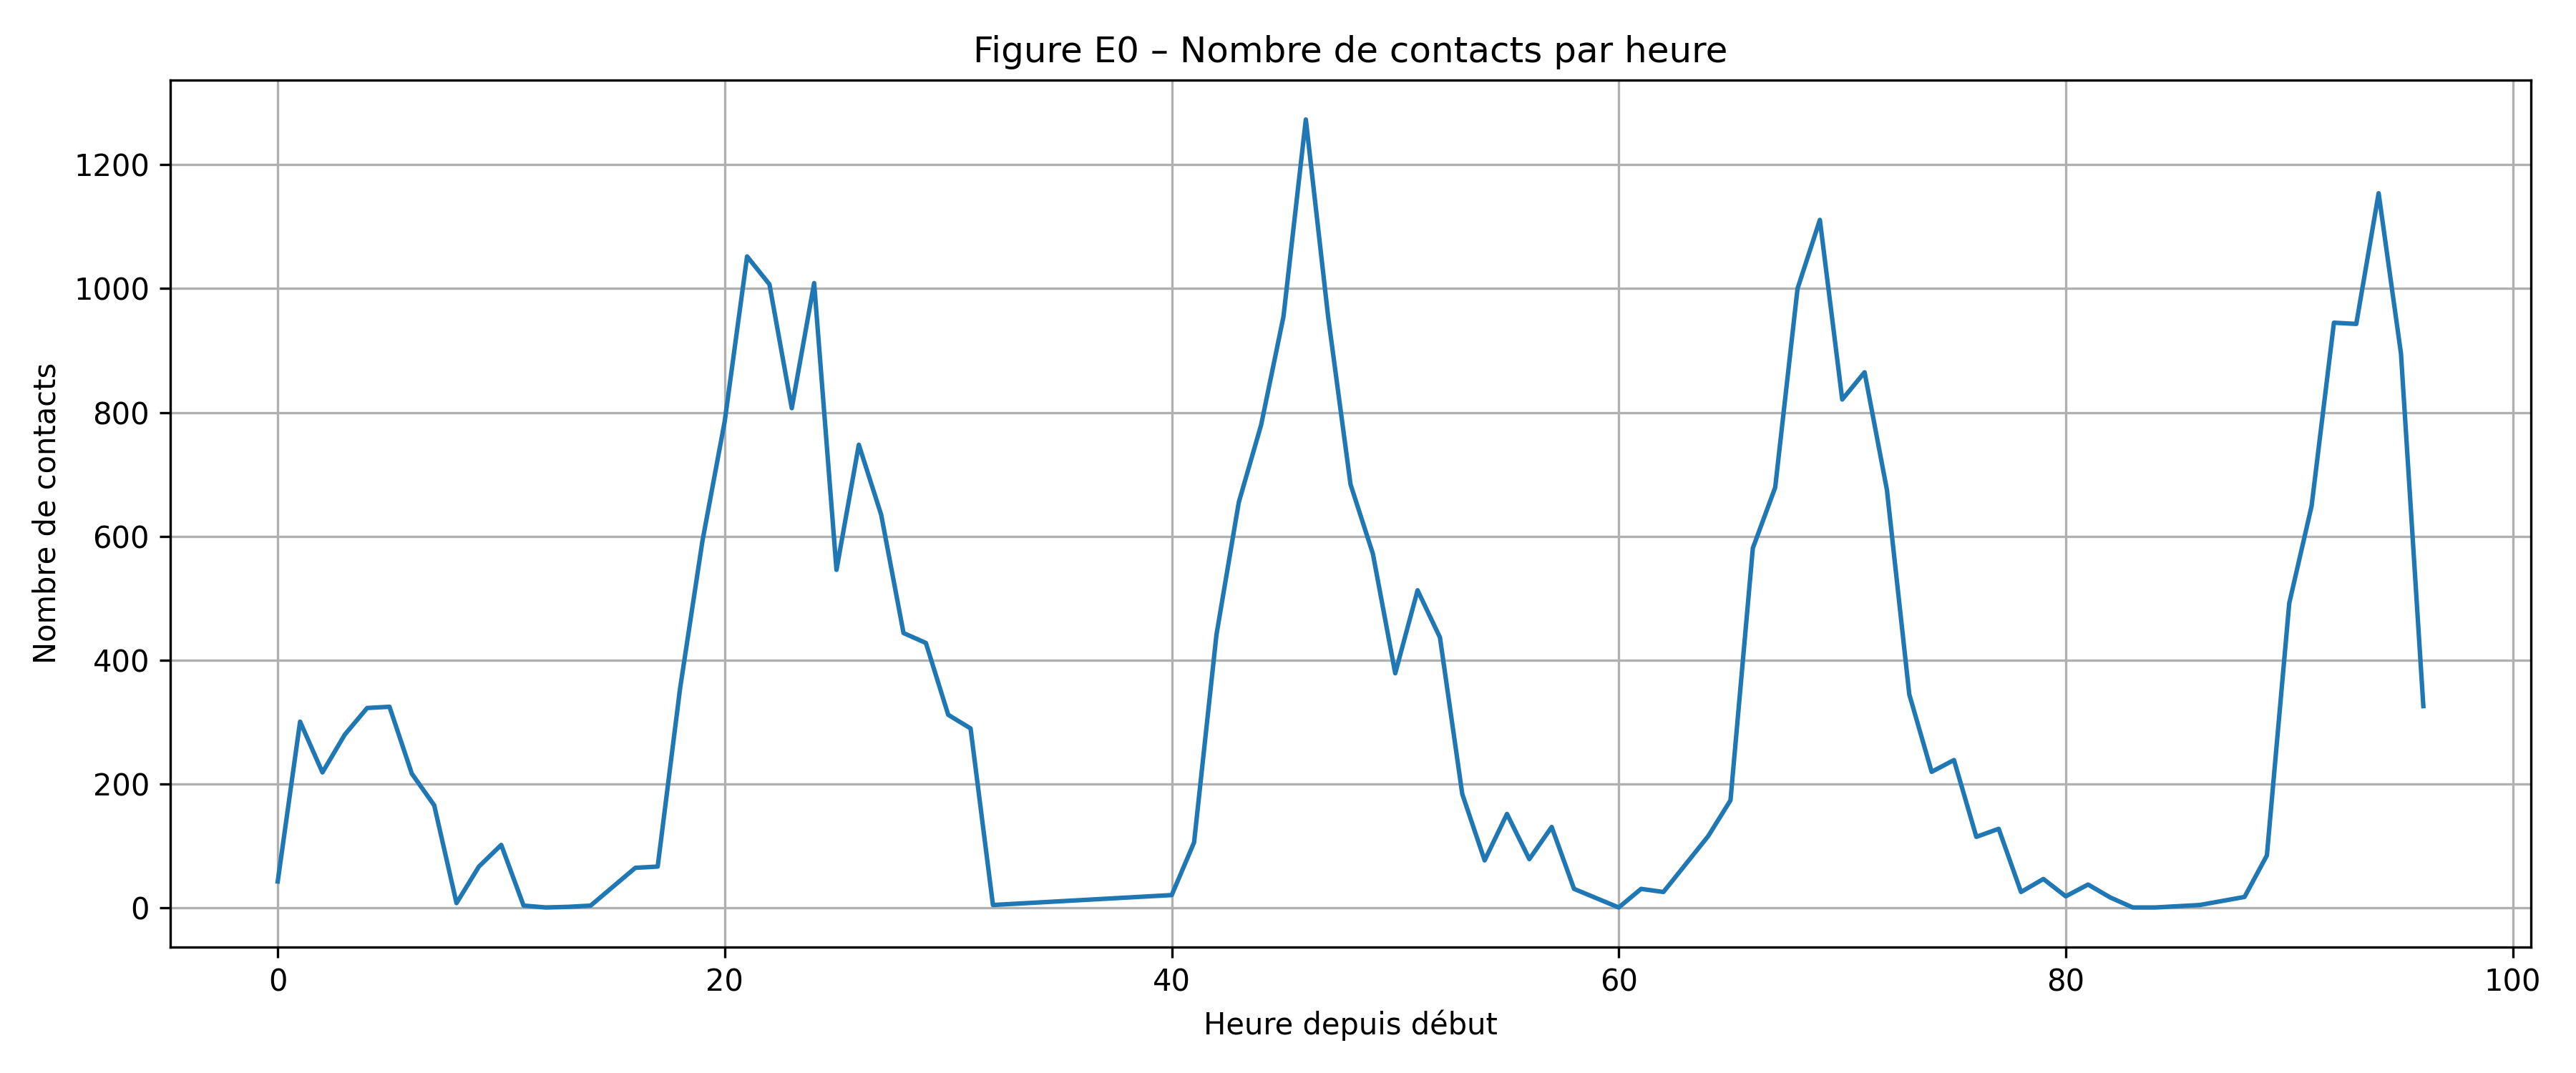
\includegraphics[width=0.90\linewidth]{images/article1/Figure_E0_contacts_par_heure.png}
\caption{Nombre total de contacts par heure.}
\end{figure}

On observe une structure \textbf{cyclique} :
pics marqués en journée (activité soignante) et creux nocturnes.  
Cela indique une organisation temporelle stable et répétitive.

\subsection{Contacts par type d’interaction}

\begin{figure}[H]
\centering
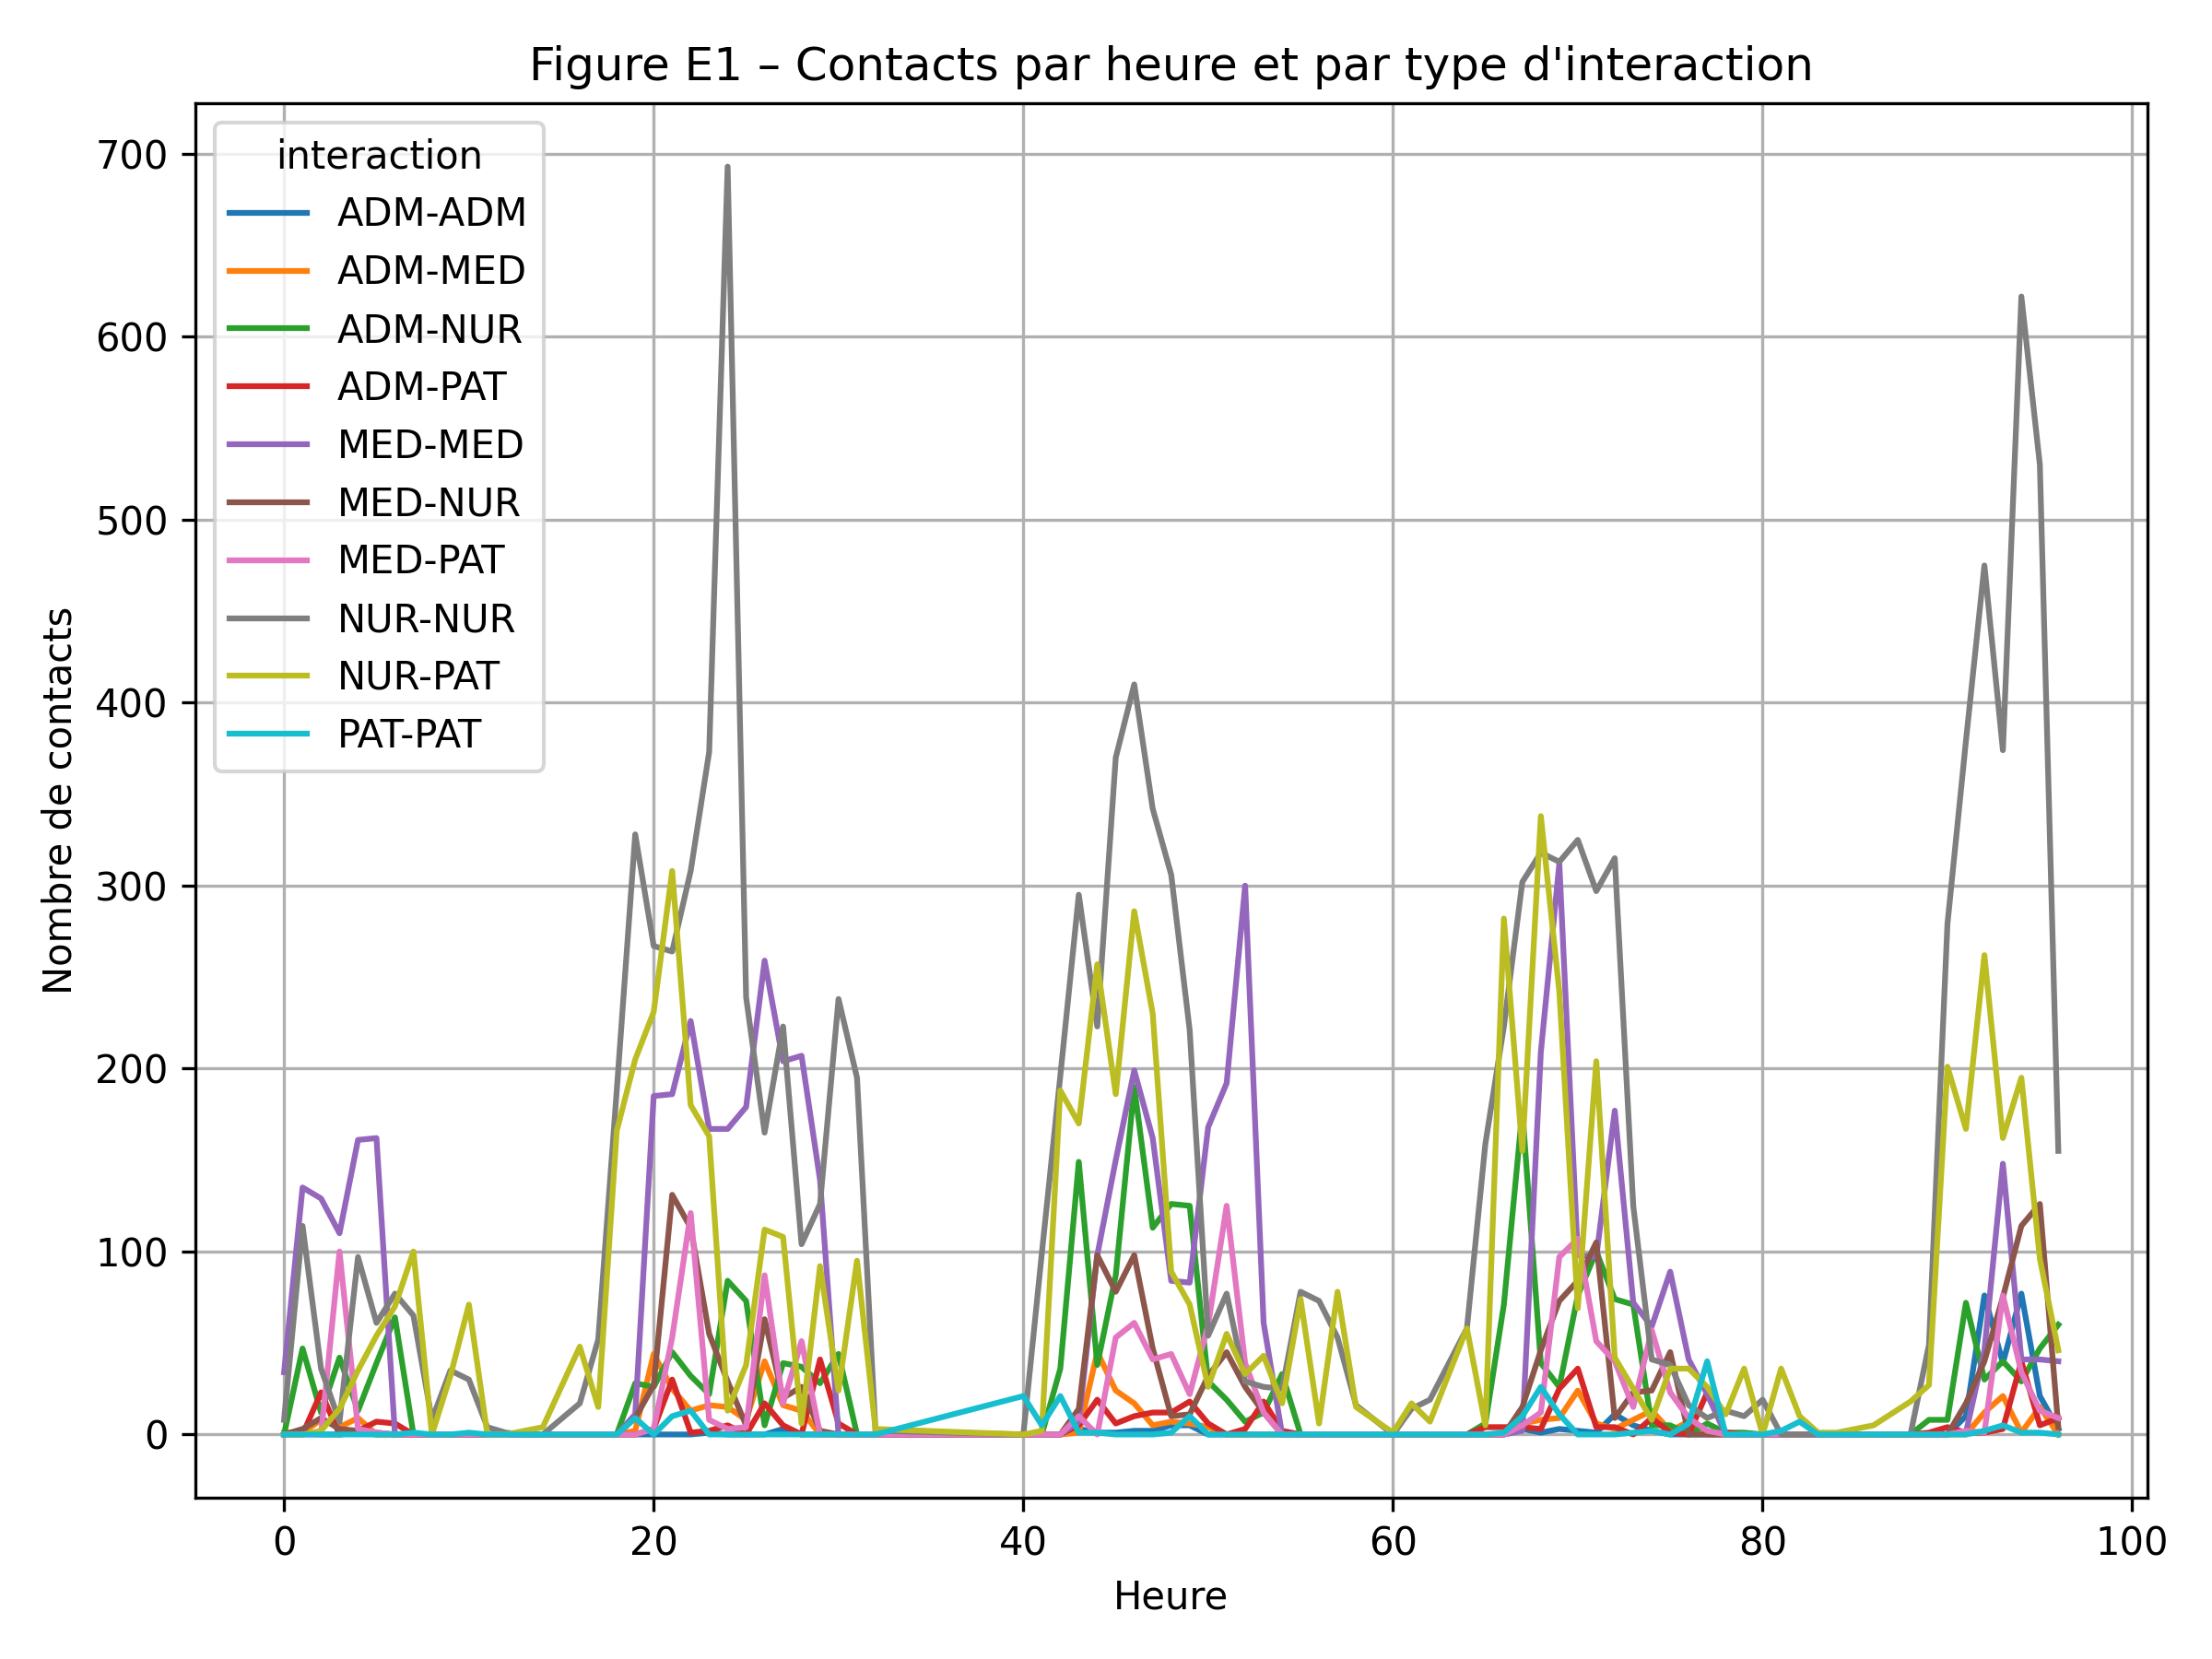
\includegraphics[width=0.90\linewidth]{images/article1/Figure_E1_contacts_par_role.png}
\caption{Contacts par heure selon le type d’interaction.}
\end{figure}

Les interactions \textbf{NUR--PAT} et \textbf{NUR--NUR} dominent :
les infirmiers sont l’interface opérationnelle entre patients et système hospitalier.  
Les \textbf{ADM} restent faibles et davantage internes à leur catégorie.

% ============================================================
\section{Stabilité du voisinage : similarité de Jaccard}
% ============================================================

\subsection{Définition}

Pour un individu $i$, si $N_1(i)$ est l’ensemble de ses voisins au jour 1 et $N_2(i)$ au jour 2 :
\[
J(i)=\frac{|N_1(i)\cap N_2(i)|}{|N_1(i)\cup N_2(i)|}.
\]


\subsection{Résultats par rôle}

\begin{figure}[H]
\centering
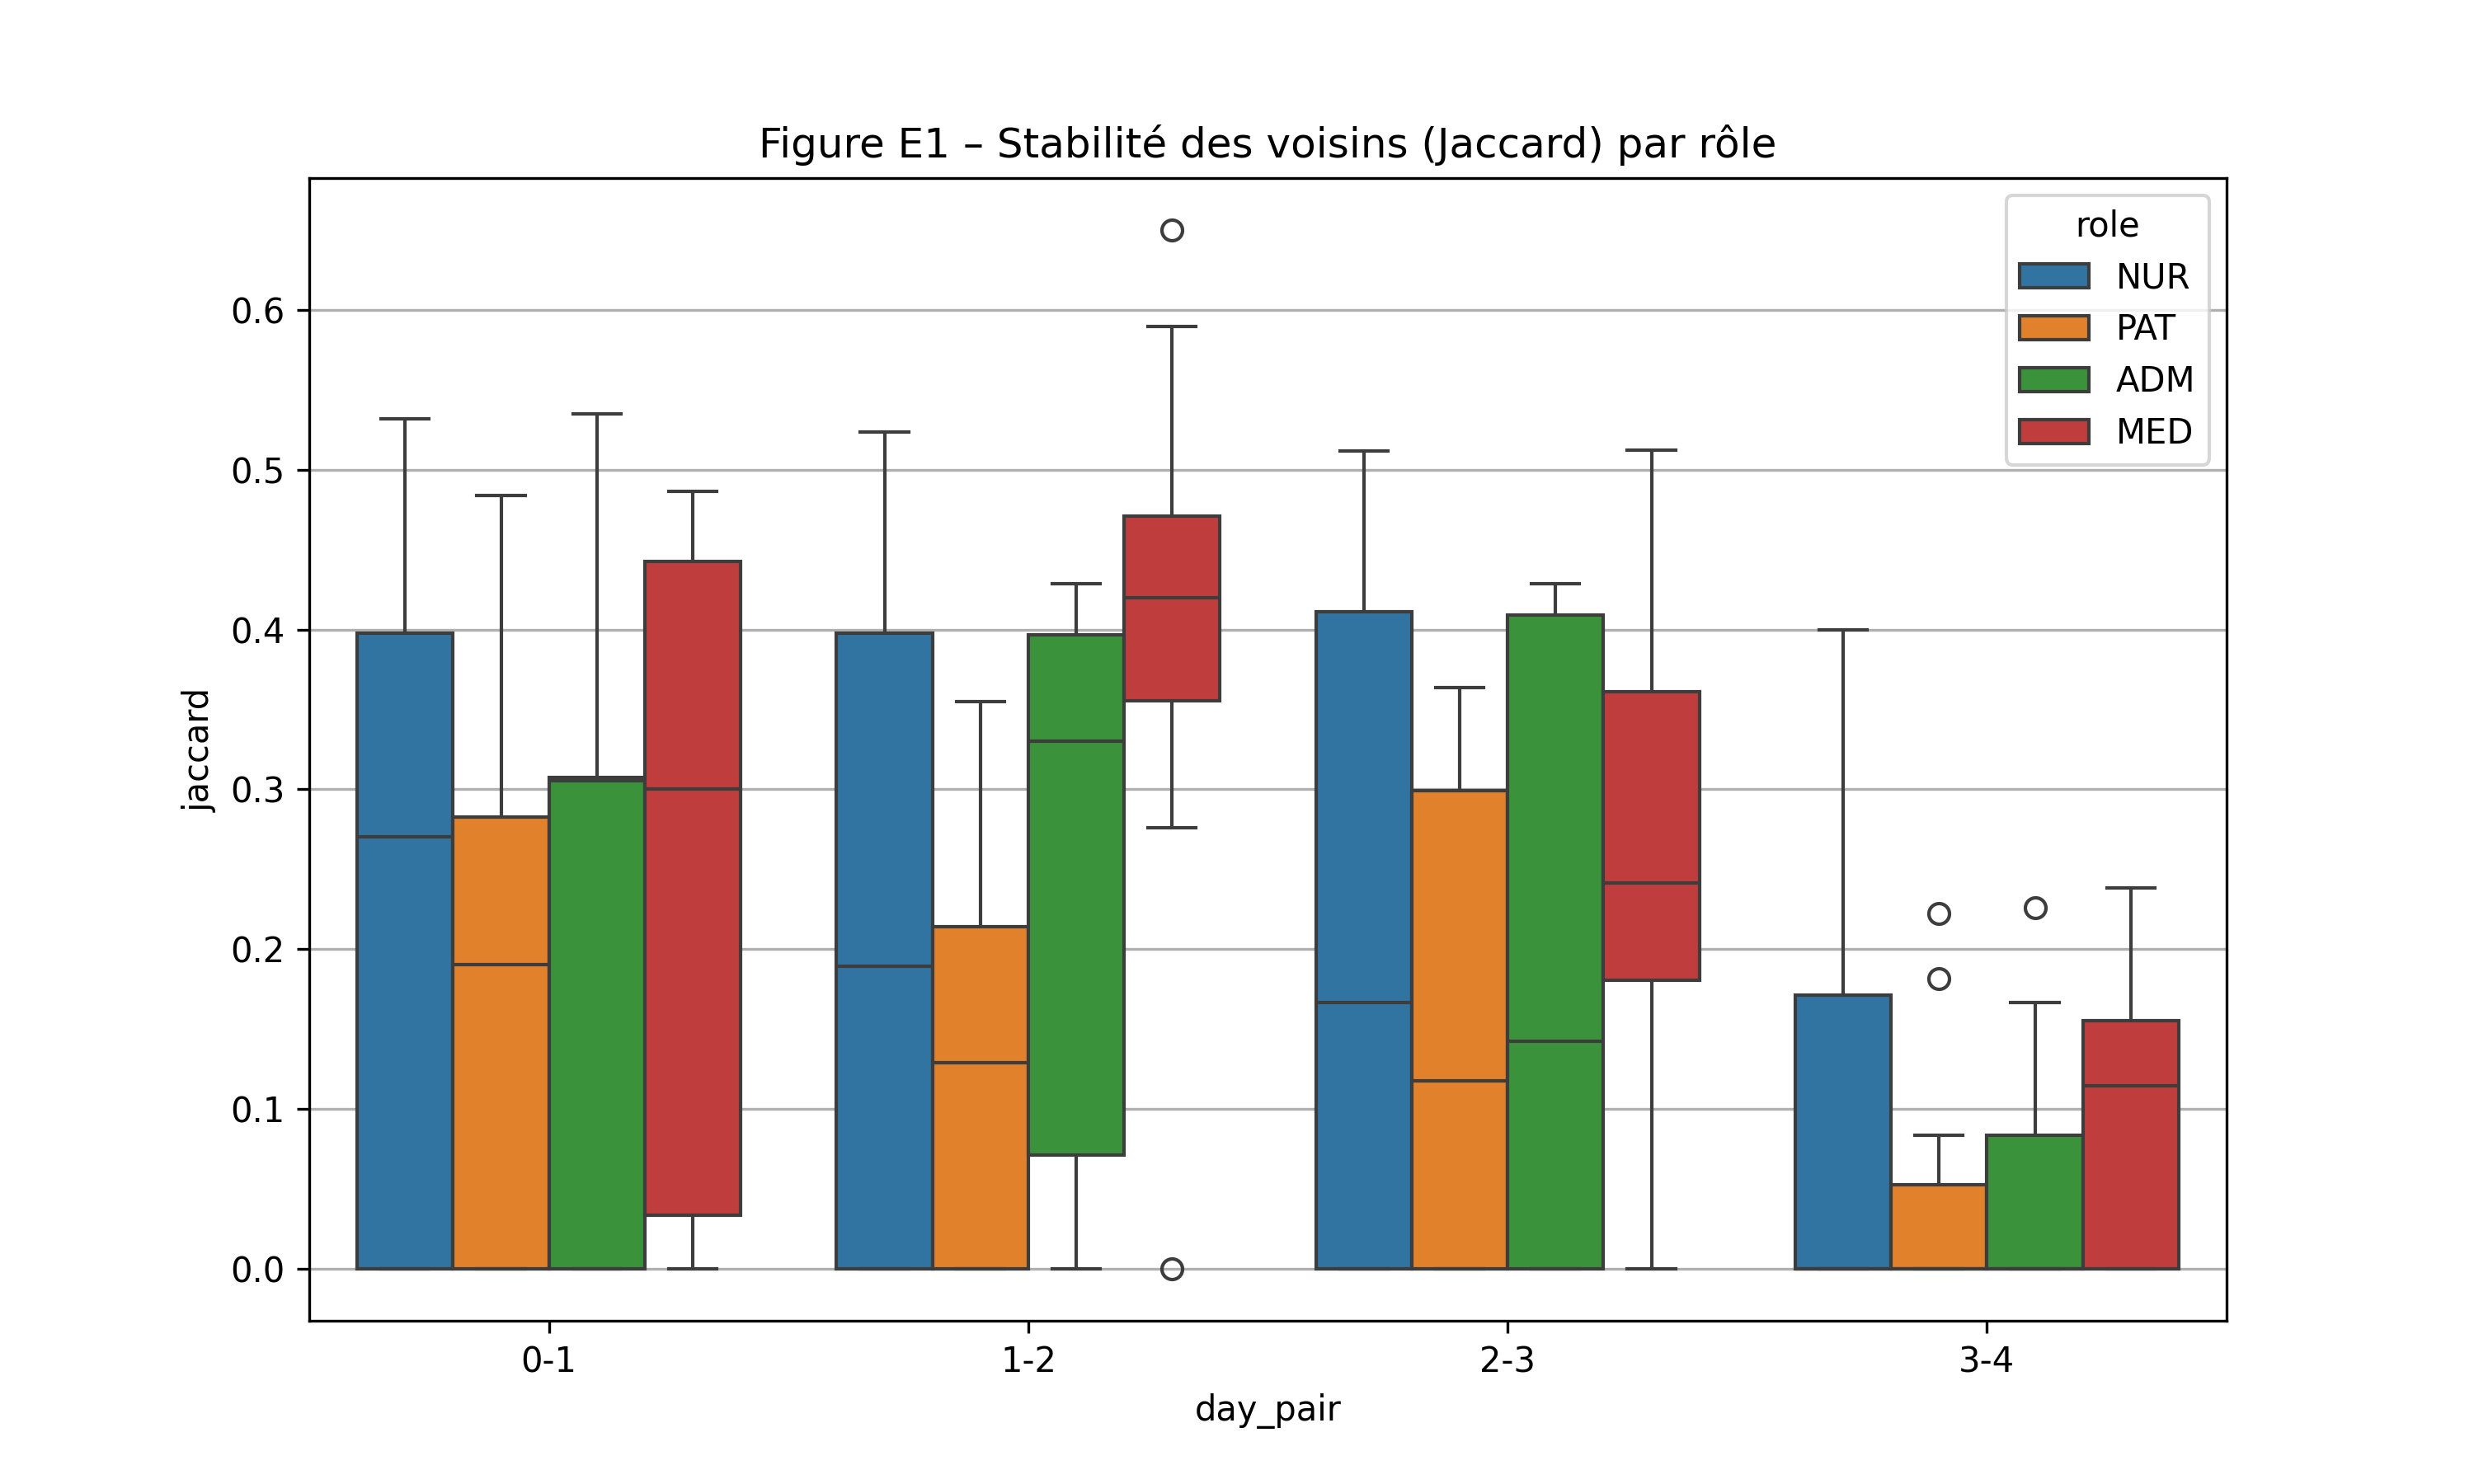
\includegraphics[width=0.85\linewidth]{images/article1/Figure_E1_stabilite_voisinage.png}
\caption{Stabilité des voisinages (Jaccard) par rôle.}
\end{figure}

\begin{itemize}
    \item \textbf{NUR} : stabilité élevée $\Rightarrow$ équipes et routines de soins.
    \item \textbf{MED} : stabilité intermédiaire.
    \item \textbf{PAT} : stabilité faible $\Rightarrow$ interactions dépendantes des soins, déplacements, état clinique.
\end{itemize}

Ainsi, le personnel présente une structure sociale stable, tandis que la partie patient est plus dynamique.

% ============================================================
\section{Structure temporelle : compacité et connectivité}
% ============================================================

On étudie ici comment la structure instantanée (par heure) évolue en termes de distances et connectivité globale.

\subsection{Diamètre}

\begin{figure}[H]
\centering
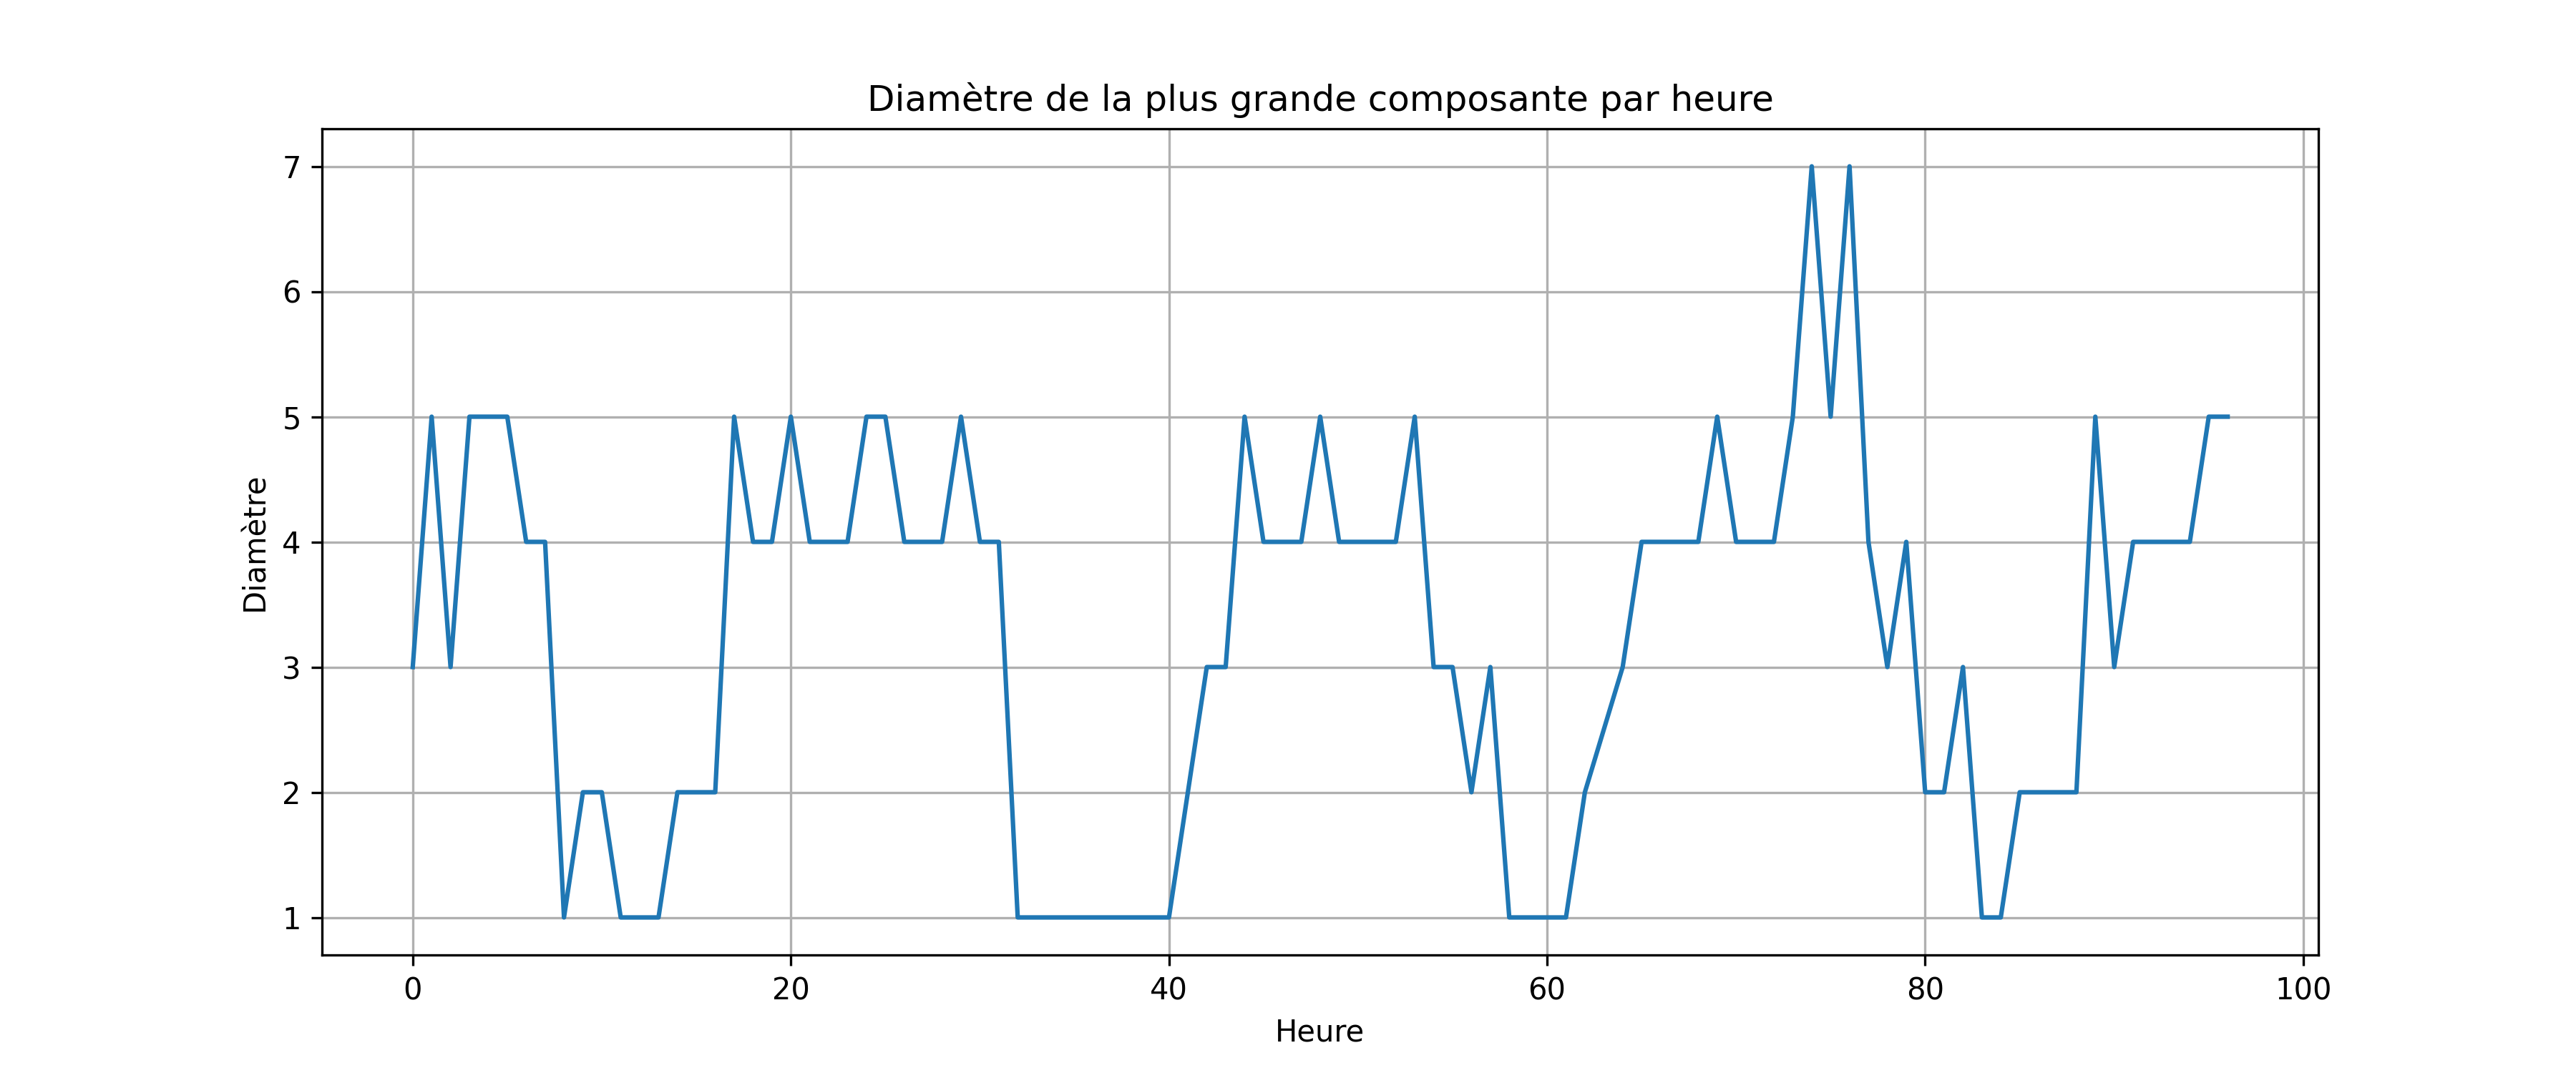
\includegraphics[width=0.90\linewidth]{images/article1/Figure_E2_diametre.png}
\caption{Diamètre de la plus grande composante.}
\end{figure}

Un diamètre entre 3 et 7 indique un réseau \textbf{compact} :
même dans les périodes moins actives, les distances restent faibles.

\subsection{Distance moyenne}

\begin{figure}[H]
\centering
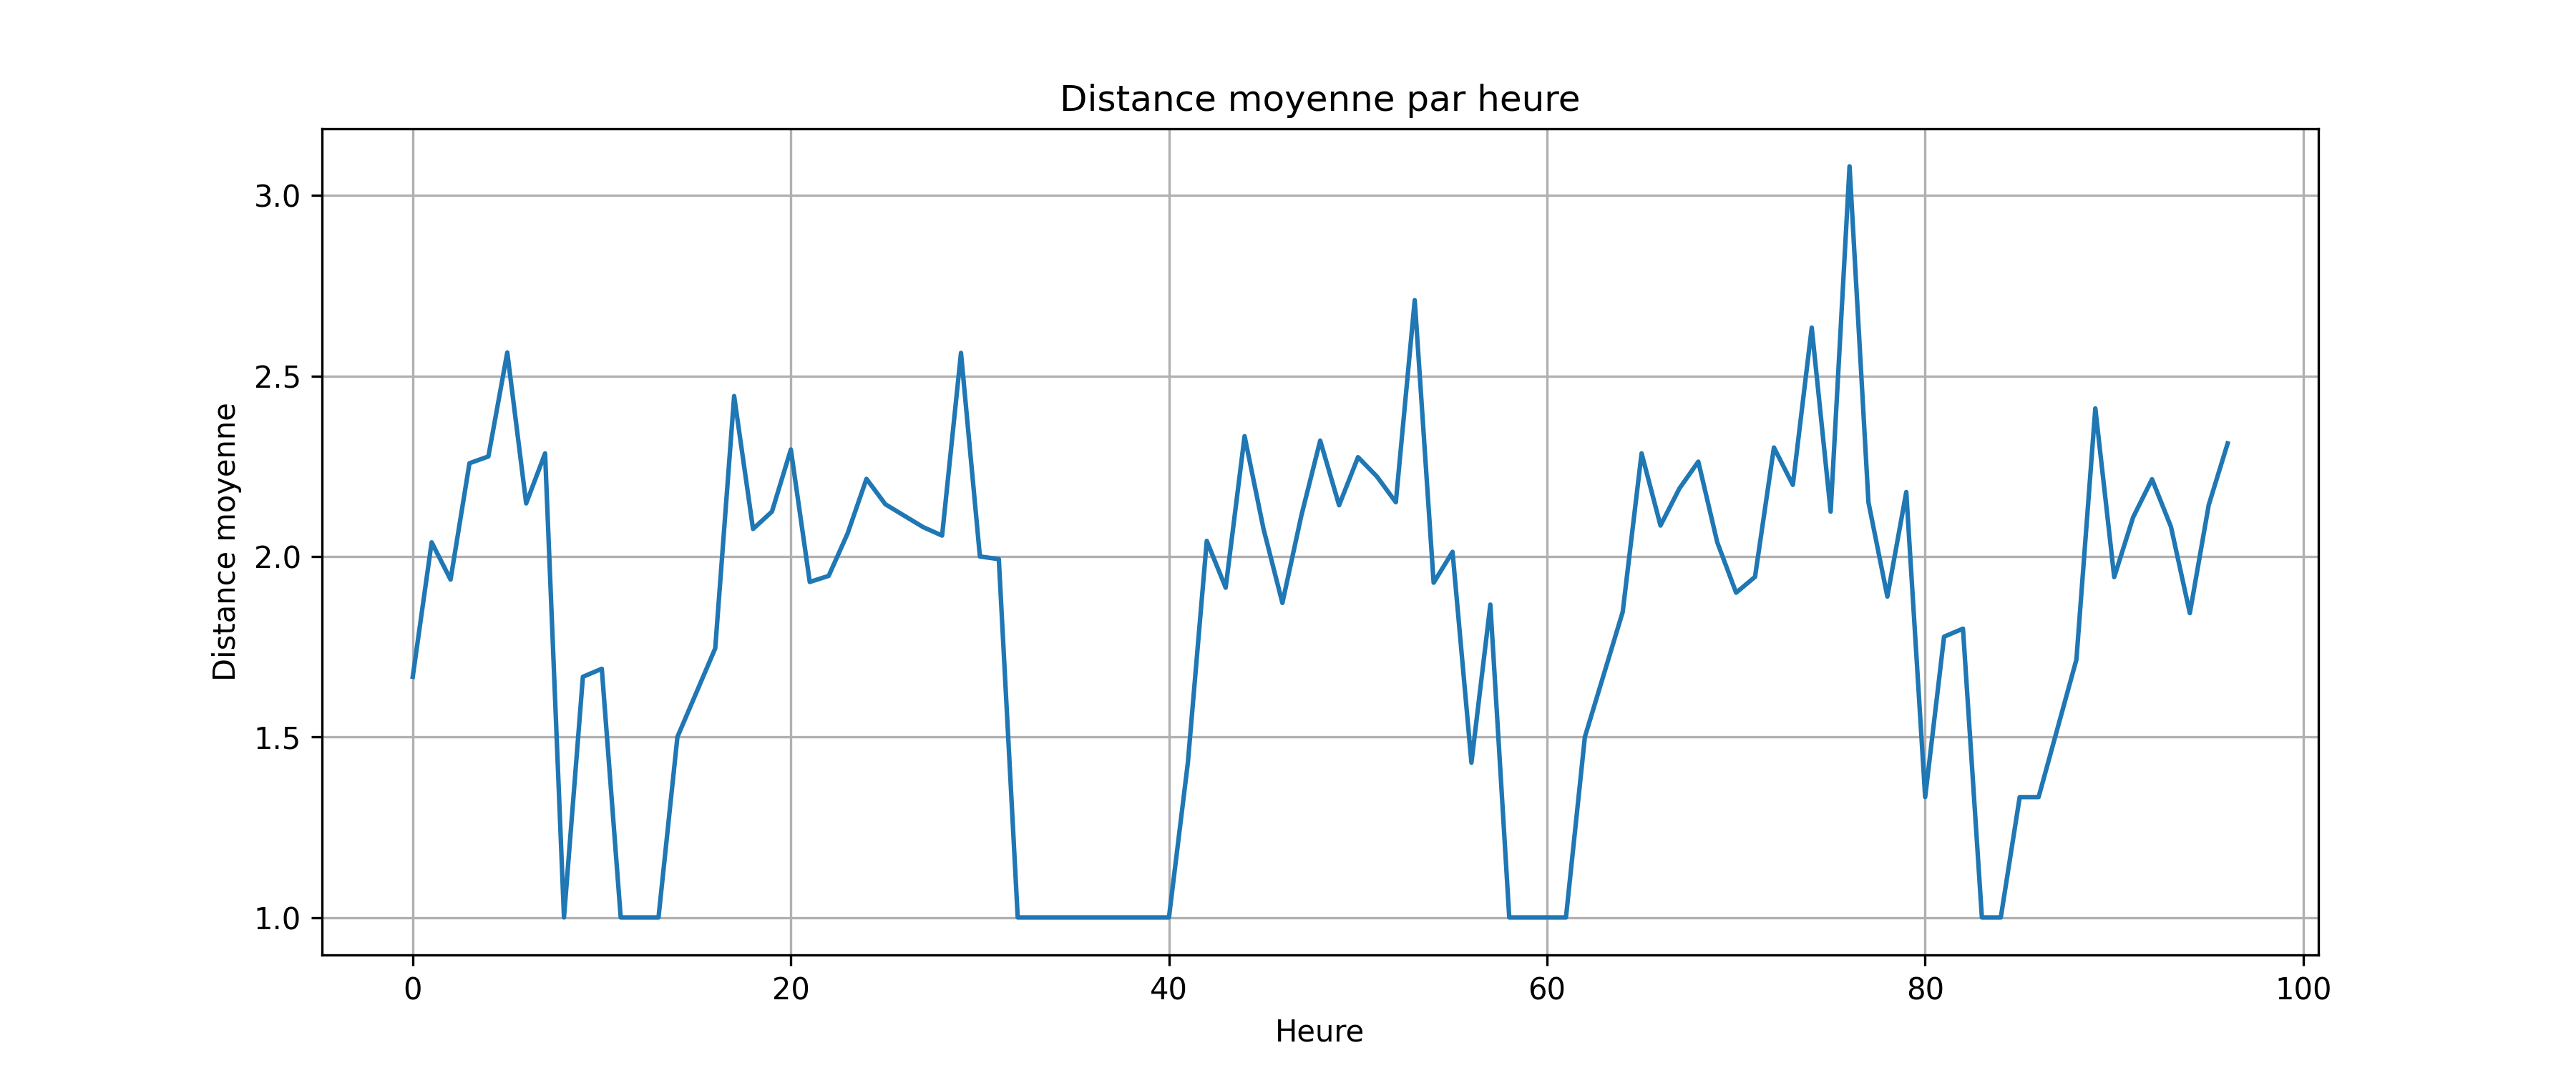
\includegraphics[width=0.90\linewidth]{images/article1/Figure_E3_distance_moyenne.png}
\caption{Distance moyenne par heure.}
\end{figure}

Avec une distance moyenne entre 1.8 et 2.6, l’information (ou un agent infectieux) peut se propager très rapidement.

\subsection{Nombre de composantes}

\begin{figure}[H]
\centering
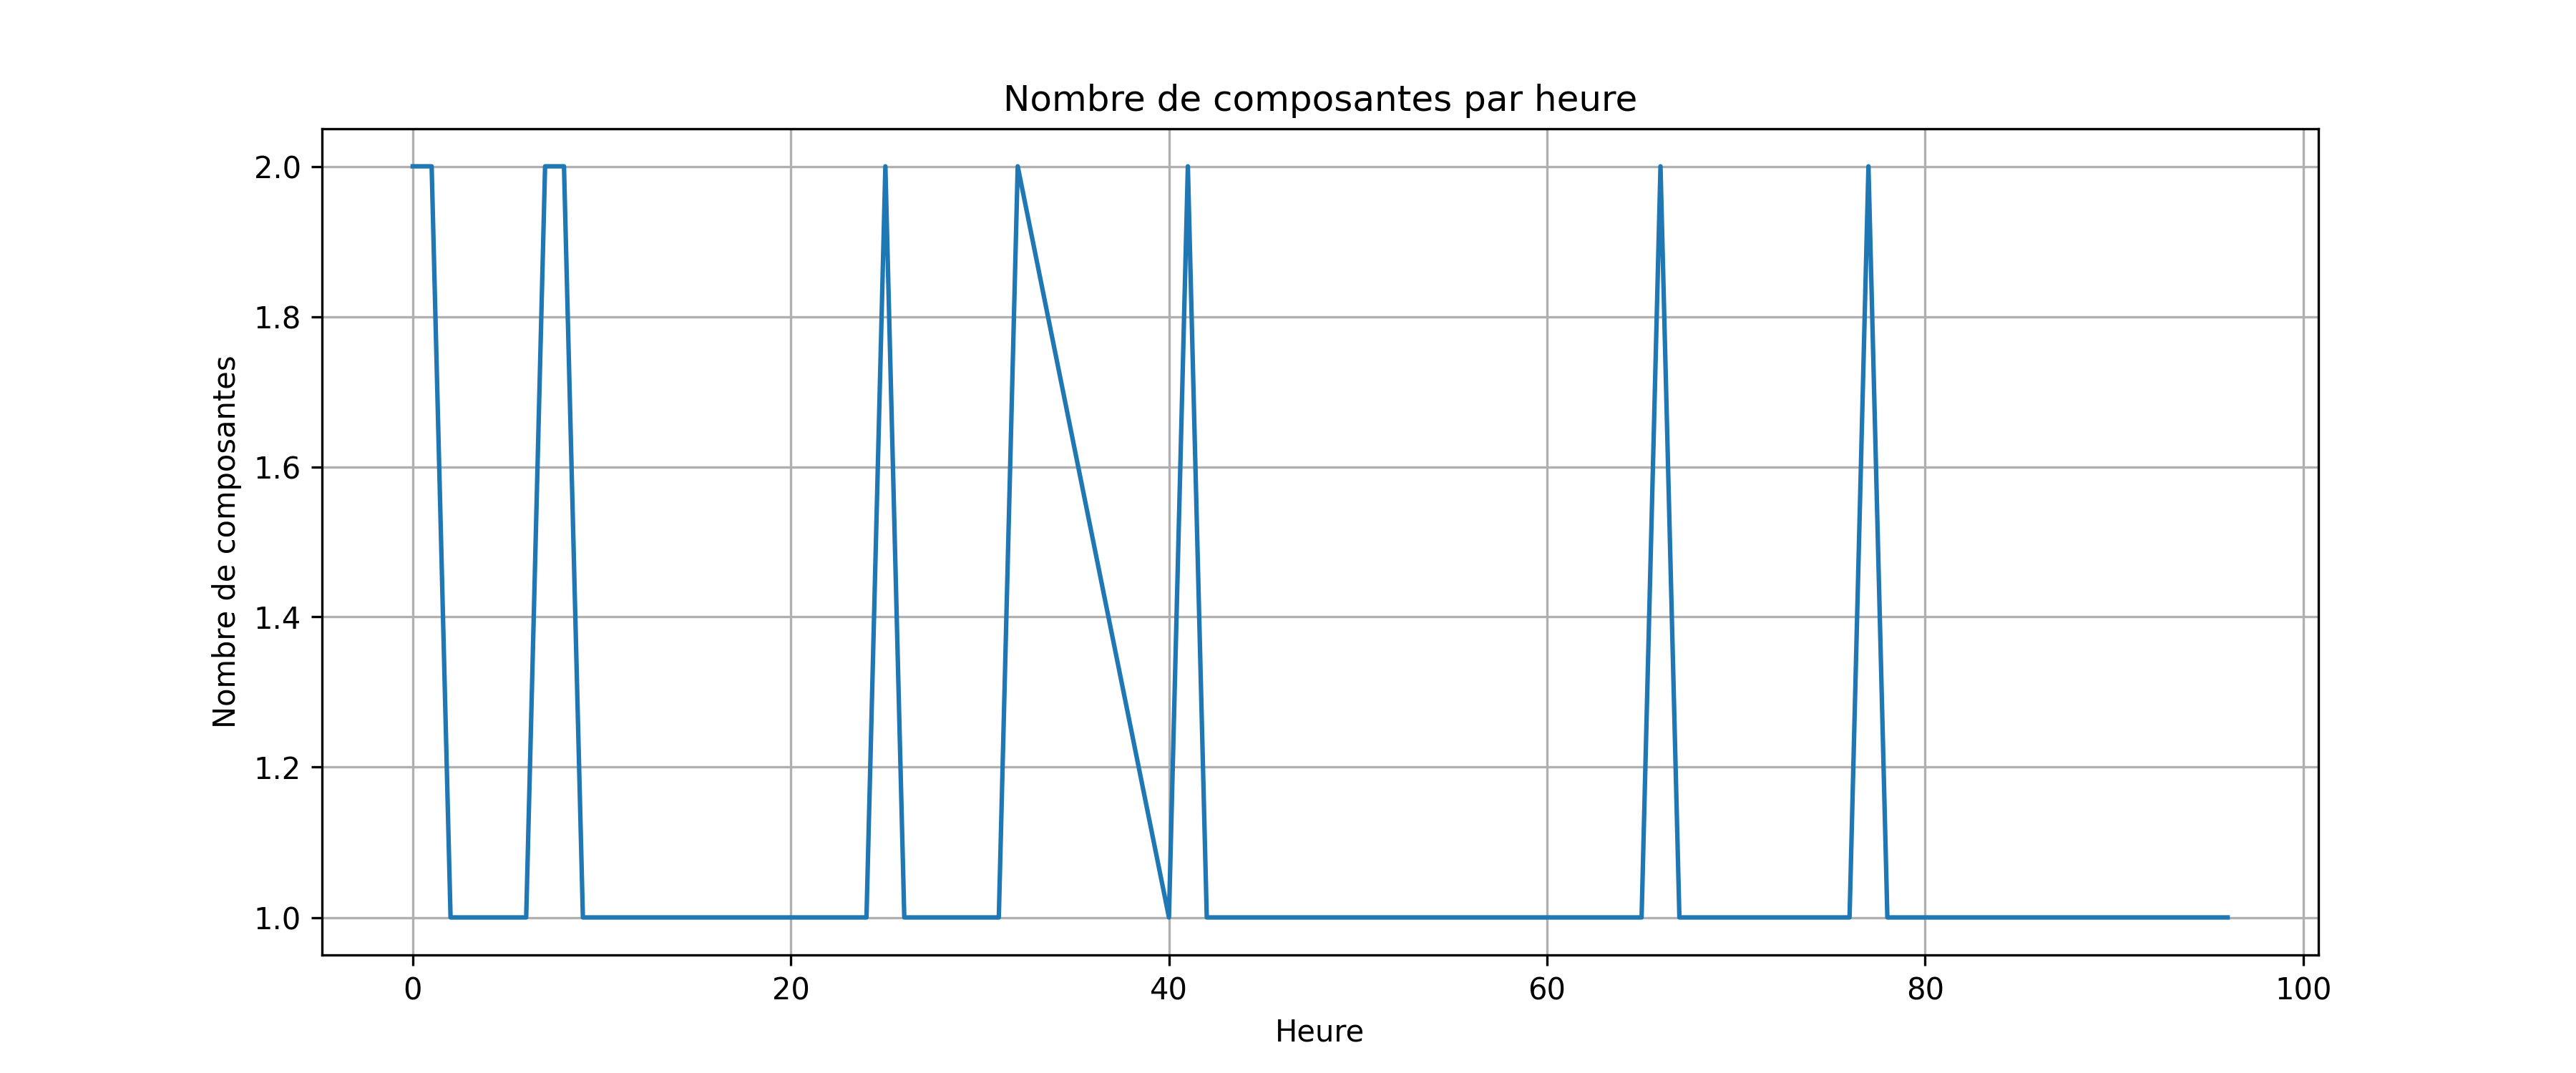
\includegraphics[width=0.90\linewidth]{images/article1/Figure_E4_composantes.png}
\caption{Nombre de composantes du graphe.}
\end{figure}

Le réseau reste quasi toujours connecté : forte cohésion structurelle, faible fragmentation.

% ============================================================
\section{Graphe agrégé : visualisation et communautés}
% ============================================================

Le graphe agrégé résume l’ensemble des contacts sur la période :
\textbf{75 nœuds} et \textbf{1139 arêtes}, donc un réseau très dense.

\subsection{Visualisation brute}

\begin{figure}[H]
\centering
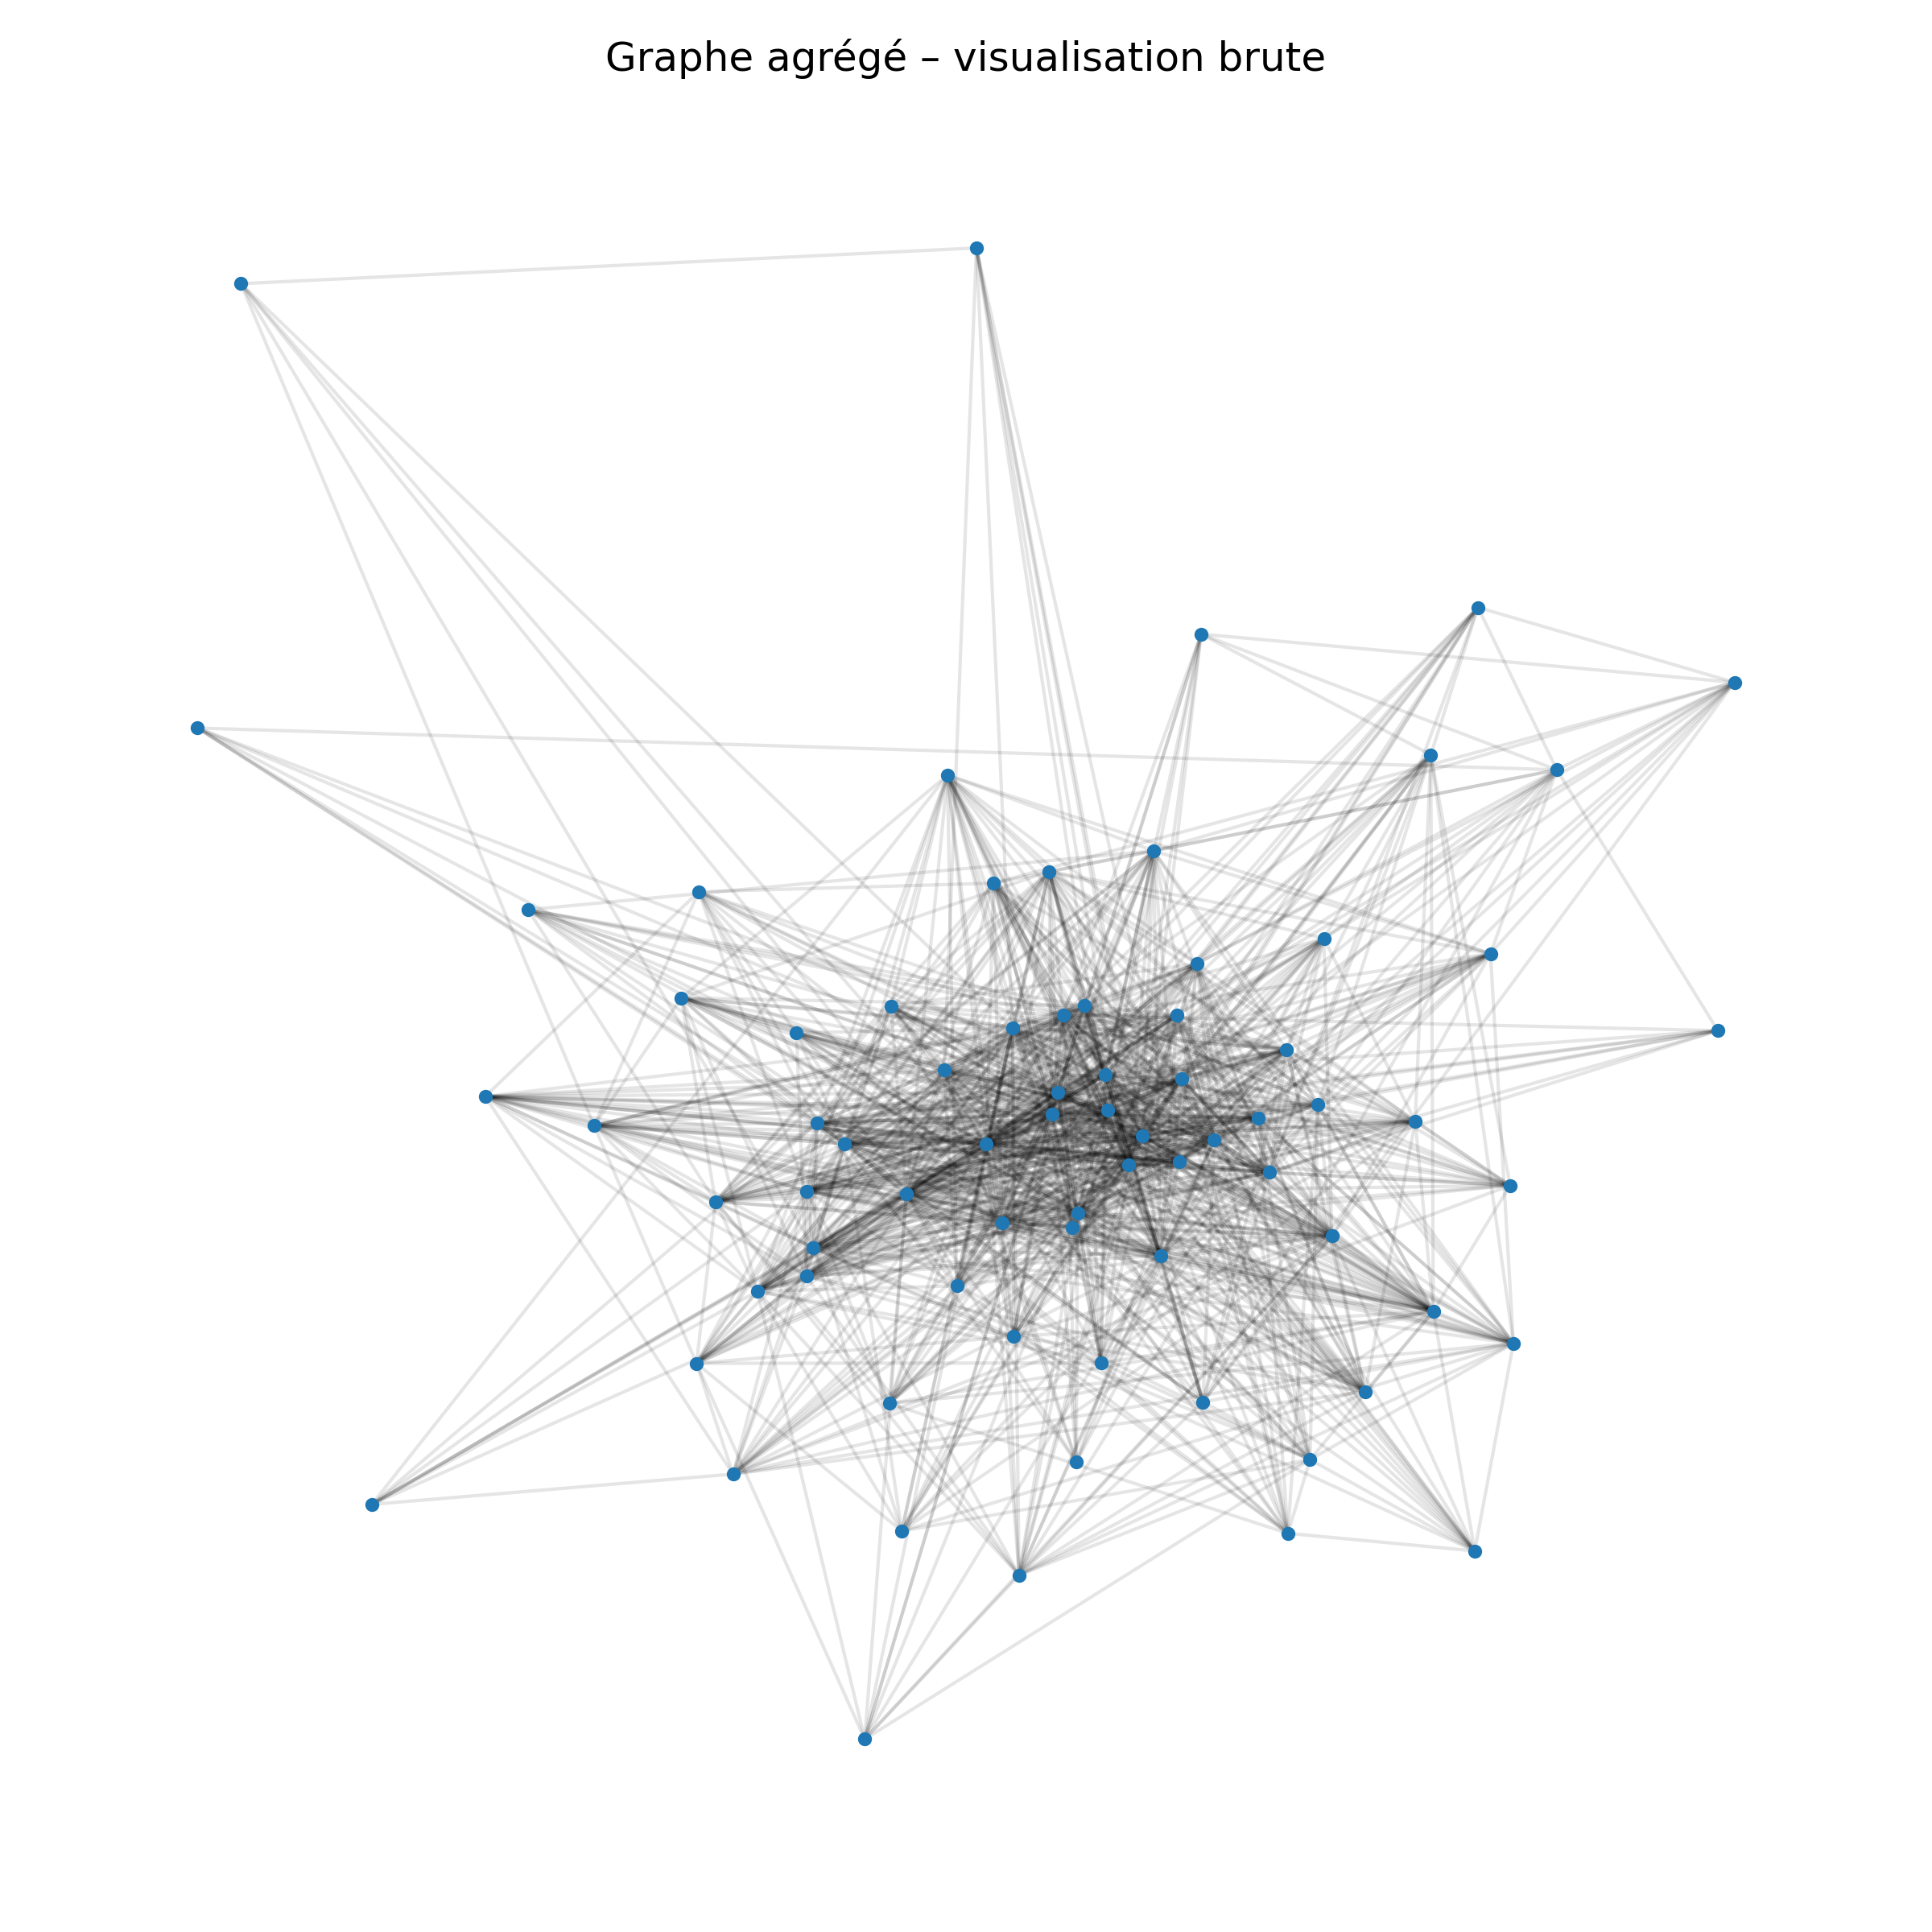
\includegraphics[width=0.75\linewidth]{images/article1/Figure_D0_graphe_brut.png}
\caption{Graphe agrégé : visualisation brute.}
\end{figure}

La densité élevée rend la zone centrale très saturée, typique d’un noyau de personnel fortement interconnecté.

\subsection{Détection de communautés (Louvain)}



\begin{figure}[H]
\centering
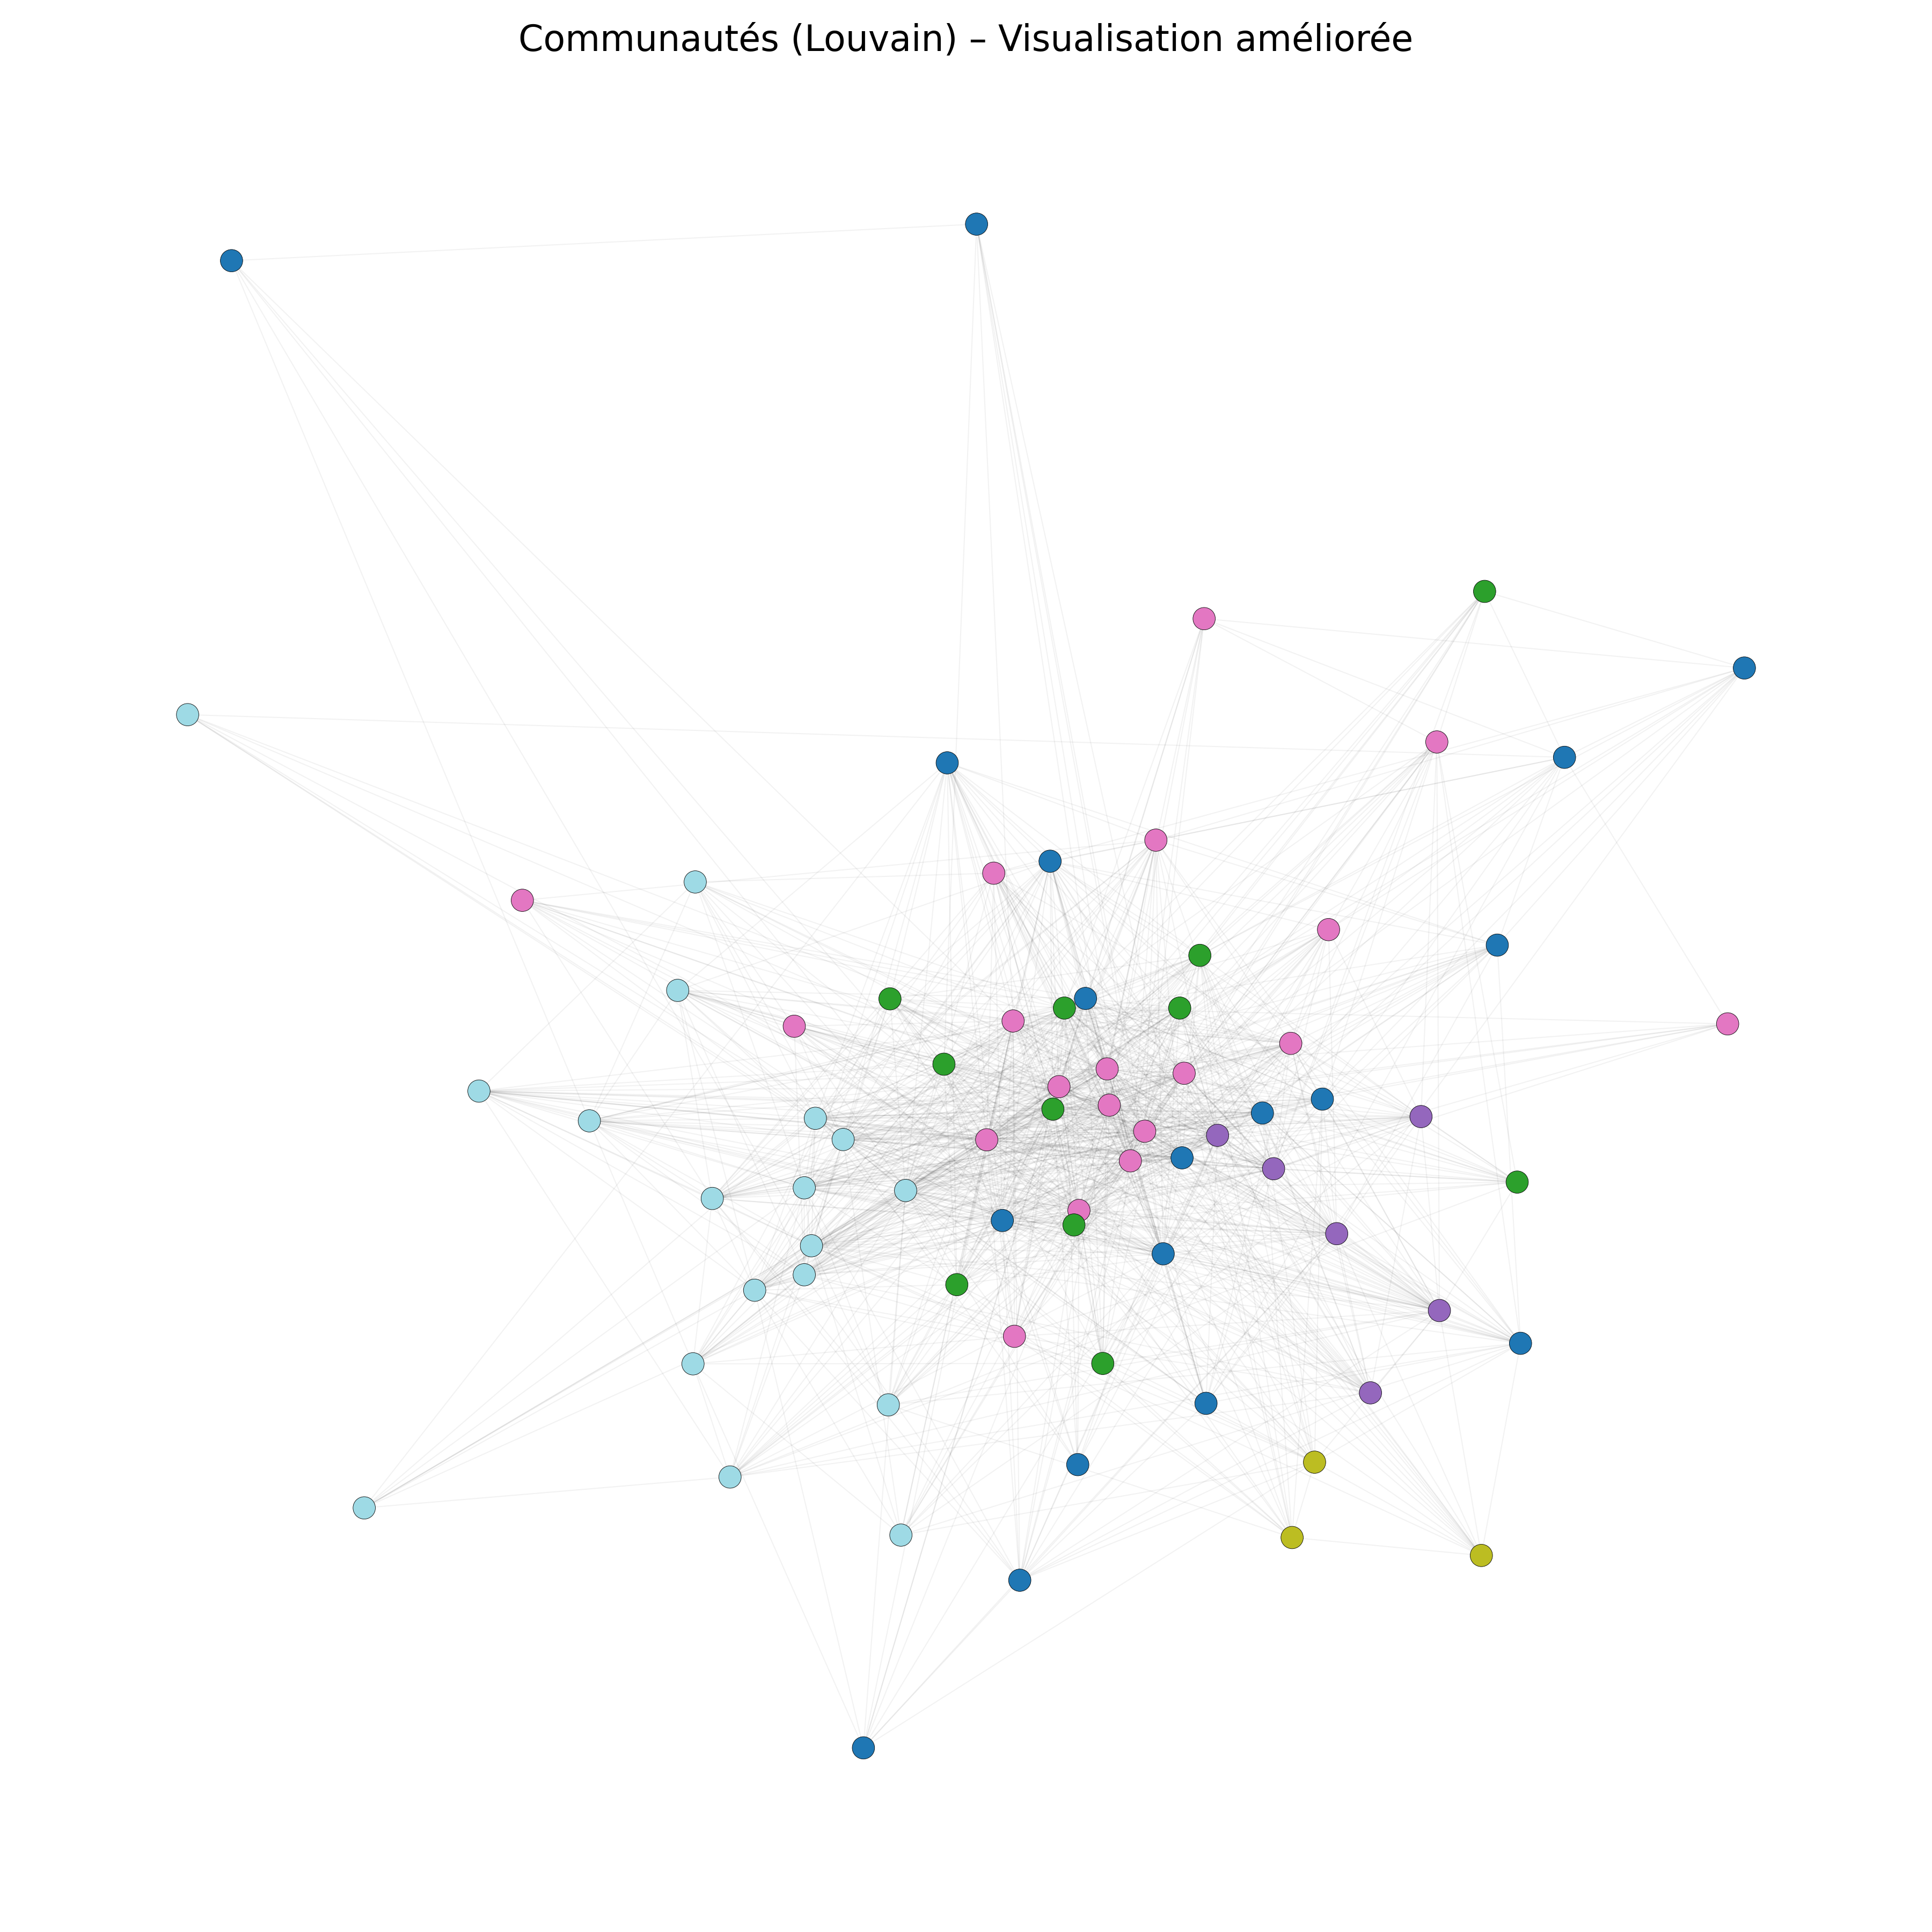
\includegraphics[width=0.75\linewidth]{images/article1/Figure_D1_communautes_améliorée.png}
\caption{Communautés détectées.}
\end{figure}

Le réseau présente \textbf{6 communautés} avec une modularité de \textbf{0.368}, indiquant une structure communautaire \textbf{modérée}.  
Ces modules correspondent plausiblement à des équipes soignantes, ou à des sous-ensembles “patients + personnel référent”.

% ============================================================
\section{Structure core--périphérie}
% ============================================================

La structure core--périphérie est identifiée à partir de la probabilité de persistance
$\alpha_S$ sur le graphe agrégé, pondéré par la fréquence des contacts.
La coupure obtenue isole une \textbf{périphérie de 74 nœuds} et un \textbf{core réduit à un seul individu}
(ID \textbf{1115}, rôle \textbf{NUR}).

La courbe $\alpha_S$ reste nulle sur la majorité des étapes, puis augmente brutalement
lorsque ce nœud est inclus, indiquant une forte centralisation des interactions.
La périphérie regroupe l’ensemble des autres rôles (patients, médecins et administratifs),
tandis que le noyau correspond à un infirmier particulièrement dominant,
en cohérence avec les résultats obtenus sur les centralités.

% ============================================================
\section{Interprétation générale}
% ============================================================

Les résultats obtenus confirment une organisation des contacts hospitaliers
fortement structurée et hétérogène.
Les analyses montrent qu’un nombre limité d’infirmiers, et dans une moindre mesure
de médecins, concentre une part importante des interactions, tant en nombre
qu’en durée, et occupe des positions centrales dans la connectivité globale du réseau.
Ces individus correspondent aux profils identifiés dans l’article comme
potentiels super-contacteurs parmi les professionnels de santé.

La comparaison avec des graphes de référence indique que cette organisation
ne peut être expliquée par le hasard ni par la seule distribution des degrés.
La présence d’un clustering élevé et de motifs d’interaction dépendants des rôles
reflète des contraintes fonctionnelles liées au fonctionnement de l’hôpital.

L’étude temporelle met en évidence des cycles journaliers marqués,
avec des pics d’activité en journée et une baisse nette la nuit,
tout en montrant une stabilité globale des patterns de contacts d’un jour à l’autre.
Enfin, l’organisation communautaire et la structure core--périphérie
révèlent un noyau dense principalement composé de soignants,
entouré d’une périphérie dominée par les patients.

Dans l’ensemble, ces observations sont cohérentes avec les conclusions de l’article
et soulignent le rôle central du personnel soignant dans la structuration
et la dynamique des contacts hospitaliers.

\end{document}